\documentclass{article} % For LaTeX2e
\usepackage[table]{xcolor}
\usepackage{nips15submit_e,times}
\usepackage{hyperref}
\usepackage{verbatim}\usepackage{url}
\usepackage[numbers]{natbib}
\usepackage[labelformat=simple]{subcaption}
\renewcommand\thesubfigure{(\alph{subfigure})}
\usepackage{multirow}
\usepackage{pgfplots, graphicx, amsmath,amsthm,amssymb,mathtools,tikz}

\usetikzlibrary{arrows.meta, shadows, arrows, positioning}
%\usepackage{color}

\definecolor{SFUred} {RGB}{131,33,37}

\title{A Neural Network Approach to Classifying Banana Ripeness}

\author{
Kyle Demeule\\
Department of Computing Science\\
Faculty of Applied Sciences\\
Simon Fraser University\\
8888 University Drive\\
\texttt{kdd2@sfu.ca} \\
\And
Bernard S Chan \\
Department of Computing Science\\
Faculty of Applied Sciences\\
Simon Fraser University\\
8888 University Drive\\
\texttt{bernardc@sfu.ca} \\
\AND
Saeed Soltani\\
Department of Computing Science\\Faculty of Applied Sciences\\
Simon Fraser University\\
8888 University Drive\\
\texttt{saeeds@sfu.ca} \\
}

% The \author macro works with any number of authors. There are two commands
% used to separate the names and addresses of multiple authors: \And and \AND.
%
% Using \And between authors leaves it to \LaTeX{} to determine where to break
% the lines. Using \AND forces a linebreak at that point. So, if \LaTeX{}
% puts 3 of 4 authors names on the first line, and the last on the second
% line, try using \AND instead of \And before the third author name.

\newcommand{\fix}{\marginpar{FIX}}
\newcommand{\new}{\marginpar{NEW}}

\nipsfinalcopy % Uncomment for camera-ready version

\begin{document}


\maketitle

\begin{abstract}
Automatic fruit ripeness detection through machine learning techniques is an active and widely applicable research topic. In this paper, a new technique to detect banana ripeness and non-banana objects is introduced. First, an appropriate data set on bananas was generated under controlled conditions. Instead of histogram or segmentation based methods, we use AlexNet, a convolution neural network model supported by Caffe, to extract features. Through the extracted features, support vector classifiers with various kernels, such as linear, radial basis functions, sigmoid and polynomial,  were used to classify the different objects. Features extracted from different exit points of AlexNet were also considered in the experiment. Overall, the combination of features extracted from FC6 and support vector classifier with radial basis function kernel provided the best results. In strictly classifying the ripeness of bananas, this combination has 90.2\% accuracy in testing. \end{abstract}

\section{Introduction}

Traditionally, humans detect ripeness of fruit  through sight, odour, taste and touch. While people and animals are naturally equipped with these senses, machines are not, so automating fruit ripeness detection is a difficult task. Given that odor sensors and image processing are more reliable and developed than taste and touch, machine learning research in detecting fruit ripeness have been based around odor and sight.  Through different type of odour sensors,~\citet{llobet1999non} and~\citet{li2007neural} collected smell information on ripening bananas and apples. Then, they applied various supervised classifier to classify their states.

Instead of odour, we are interested in integrating imaging and deep learning techniques to classify the ripeness of bananas. Based on reviews by~\citet{dadwal2012color} and~\citet{kodagali2012computer}, typical computer vision based ripeness detection methods are based on histogram matching or image segmentation. For example,~\citet{paulraj2009color} proposed a histogram-based neural network classifier for evaluating ripeness banana. Each image in the data set is decomposed into its RGB component and the number of pixels in each channel of varying intensities were counted. This information is then vectorized and fed into an neural network to be classified as unripe, ripe, or overripe. Segmentation based methods build on top of histogram-based methods. As mentioned in~\citet{dadwal2012color}, images are preprocessed so that the fruits in the picture are separated from the rest of the image. Then, classifying techniques, such as histogram-based neural network or clustering, are applied to classifying the ripeness. Segmentation based techniques are theoretically superior because features used for classification are only extracted from the relevant segmented region. 

With the works we have reviewed, the models only classify ripeness of fruits. In application, it is likely that there are other objects aside from the fruits on interest. Therefore, our first goal for this project is to implement a new method that could detect the ripeness of bananas. Secondly, our model will differentiate between banana and non-banana objects. Because the data sets from~\citet{paulraj2009color} is not available, our initial task is to create an appropriate data set. Then, instead of using histogram or segmentation based methods, we will use convolutional neural network (CNN) to extract features. With the features of each image at hand, we construct support vector machine (SVM) classification model to classify ripeness and whether the object in question is a banana. 

The remainder of this paper is organized as follows. In Section~\ref{sec:method}, we detail the steps in data generation, features extraction and label classification. The results from our experiment are discussed in Section~\ref{sec:results} and we conclude the paper with a discussion on our results and future work in Section~\ref{sec:conclusion}. 

\begin{comment}
\section {Background}
\begin{itemize}
\item literature review on fruit ripeness
\item literature review on neural network, deep learning, AlexNet
\item introduction to technologies used (Caffe, ScikitLearn)
\end{itemize}
\end{comment}
\section{Methodology}
\label{sec:method}
For this project, we created our own data set on banana and non-banana objects because the previous data sets from~\citet{saad2009recognizing} and~\citet{paulraj2009color} were not available. After establishing our own data set, we extracted the features of the images using a pre-trained convolution neural network. The Caffe deep learning frame work by~\citet{jia2014caffe} allowed us to access to many existing models. Given that we have a visualization task with different types of objects, we chose AlexNet by~\citet{krizhevsky2012imagenet} to extract the features. After obtaining the features of the images, we used the SVM library provided in SciKit Learn~\citep{scikit-learn} to classify the objects. A workflow of this project is shown as a flowchart in Figure~\ref{fig:flowchart}. In this section, we will discuss the details in each step of our work. 

\tikzstyle{block} = [rectangle, draw, fill=SFUred!20, 
    text width=30em, text centered, rounded corners, minimum height=2em]
    \tikzstyle{small} = [rectangle, draw, fill=white!20, 
    text width=5em, text centered, rounded corners, minimum height=2em]
        \tikzstyle{medium} = [rectangle, draw, fill=white!20, 
    text width=8em, text centered, rounded corners, minimum height=2em]

\tikzstyle{line} = [draw, -latex']

\begin{figure} [h]
\centering 
{
\begin{tikzpicture}[node distance = 1.2cm, auto,scale=.1]
    % Place nodes
    \node [block] (capture) {Capture images};
    \node [block, below of=capture] (process) {Label and process images (crop, resize and convert to RGB)};
%    \node [block, below of=process] (convert) {Convert to RGB };
    \node [block, below of= process] (cnn) {Extract features via CNN (Caffe and AlexNet)};
    \node [block, below of=cnn] (svm) {Classify data via SVM (SciKit Learn)};
    \node [medium, below left = 1cm and -10cm of svm] (nonbanana) {Non-Banana};
    \node [small, below right = 1.cm and -10 cm of svm] (banana) {Banana};
    \node [small, below of = banana] (ripe) {Ripe};
    \node [small, below left = . cm and .9 cm of banana] (unripe) {Unripe};
     \node [small, below right = .cm and .9 cm of banana] (overripe) {Overripe};

    % Draw edges
    \path [line] (capture) -- (process);
    \path [line] (process) -- (cnn);
%    \path [line] (convert)--(cnn);
    \path [line] (cnn)--(svm);
    \path [line] (svm)--(nonbanana);
        \path [line] (svm)--(banana);
          \path [line] (banana)--(unripe);
        \path [line] (banana)--(overripe);
	\path [line] (banana)--(ripe);
\end{tikzpicture}
}
\caption{A flow chart of project development.}
\label{fig:flowchart}
 \end{figure}


\subsection{Generating and Preparing the Data set}

Since the data sets used by~\citet{saad2009recognizing} and~\citet{paulraj2009color} were not publicly available, we decided to create on our own data set. Controlling for lighting, background and camera (Canon S90), we took pictures of banana and various non-banana objects. After the pictures were taken, we incorporated each picture at $0\,^{\circ}$, $90\,^{\circ}$, $180\,^{\circ}$ and  $270\,^{\circ}$ of rotation to increase the number of pictures in the data set by four fold. Also, there were equal number of pictures for each of the four labels: unripe banana, ripe banana, overripe banana and non-banana. For the banana data set, twelve unique bananas were used. We used apples, tomatoes, lemons, limes, mushrooms, broccolis, potatoes, pears and green peppers as non-banana objects. In total, there were 928 images generated for the data set and sample pictures of this data set are shown in Figure~\ref{fig:sampleDataset}. After obtaining the data set, we used various Python scripts to standardize the images so that each one is resized and cropped to $256\times 256$ pixels, and applied the class labels manually. Furthermore, each picture is decomposed into the RGB channels for features extraction. 

\begin{figure}[h]
\centering
 %%%%%% unripe %%%%%%%%%
  \begin{subfigure}{.123\textwidth}
  \centering
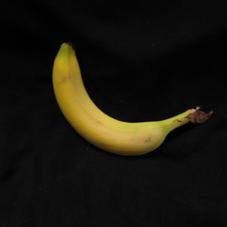
\includegraphics[width=\textwidth]{1_1.jpg}
\end{subfigure}%
 \begin{subfigure}{.123\textwidth}
  \centering
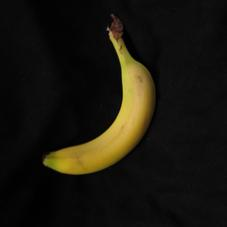
\includegraphics[width=\textwidth]{1_2.jpg}
\end{subfigure}%
  \begin{subfigure}{.123\textwidth}
  \centering
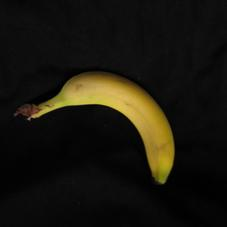
\includegraphics[width=\textwidth]{1_3.jpg}
\end{subfigure}%
  \begin{subfigure}{.123\textwidth}
  \centering
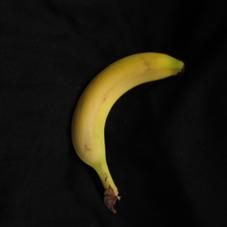
\includegraphics[width=\textwidth]{1_4.jpg}
\end{subfigure}\, %%%%%% ripe %%%%%%%%%
  \begin{subfigure}{.123\textwidth}
  \centering
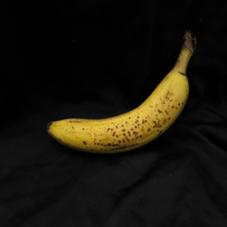
\includegraphics[width=\textwidth]{2_1.jpg}
\end{subfigure}%
 \begin{subfigure}{.123\textwidth}
  \centering
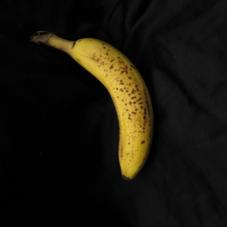
\includegraphics[width=\textwidth]{2_2.jpg}
\end{subfigure}%
  \begin{subfigure}{.123\textwidth}
  \centering
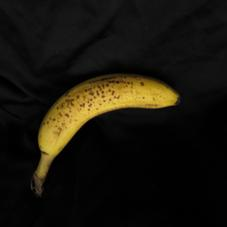
\includegraphics[width=\textwidth]{2_3.jpg}
\end{subfigure}%
  \begin{subfigure}{.123\textwidth}
  \centering
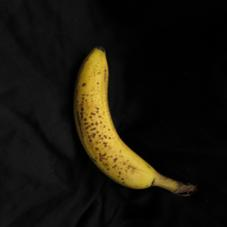
\includegraphics[width=\textwidth]{2_4.jpg}
\end{subfigure}%
\vskip .05in
 %%%%%% overripe %%%%%%%%%
  \begin{subfigure}{.123\textwidth}
  \centering
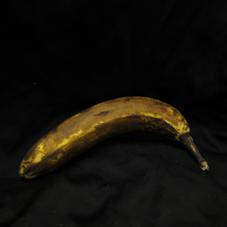
\includegraphics[width=\textwidth]{0_1.jpg}
\end{subfigure}%
 \begin{subfigure}{.123\textwidth}
  \centering
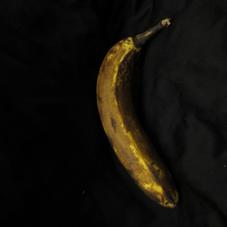
\includegraphics[width=\textwidth]{0_2.jpg}
\end{subfigure}%
  \begin{subfigure}{.123\textwidth}
  \centering
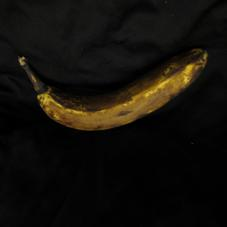
\includegraphics[width=\textwidth]{0_3.jpg}
\end{subfigure}%
  \begin{subfigure}{.123\textwidth}
  \centering
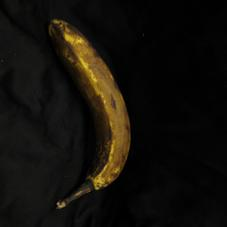
\includegraphics[width=\textwidth]{0_4.jpg}
\end{subfigure}\,
 %%%%%% non banana %%%%%%%%%
  \begin{subfigure}{.123\textwidth}
  \centering
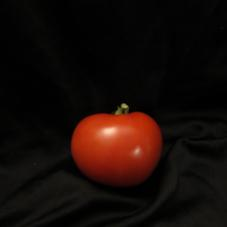
\includegraphics[width=\textwidth]{3_1.jpg}
\end{subfigure}%
 \begin{subfigure}{.123\textwidth}
  \centering
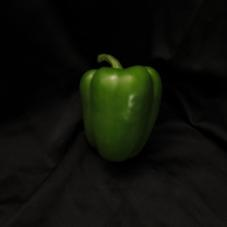
\includegraphics[width=\textwidth]{3_5.jpg}
\end{subfigure}%
  \begin{subfigure}{.123\textwidth}
  \centering
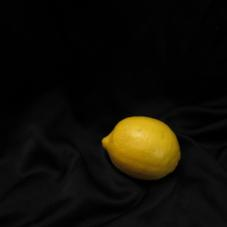
\includegraphics[width=\textwidth]{3_17.jpg}
\end{subfigure}%
  \begin{subfigure}{.123\textwidth}
  \centering
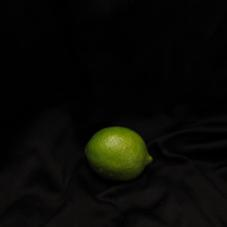
\includegraphics[width=\textwidth]{3_13.jpg}
\end{subfigure}%
\caption{Upper left: unripe bananas. Upper right: ripe bananas. Lower left: overripe bananas. Lower Right: non-banana objects.}
\label{fig:sampleDataset}
\end{figure}

 
\subsection{Features Extraction via AlexNet}

To better classify the images, a CNN was used to extract features so that other classification methods could later be used. CNNs are neural networks in which each neuron in a layer is connected to a small, adjacent portion of the previous layer. These adjacent portions overlap, so each neuron on the previous layer is connected to multiple neurons on the next, but significantly less than if the layers were fully connected. AlexNet by~\citet{krizhevsky2012imagenet} is a CNN that was developed for image classification. It was trained on 1.2 million high resolution images from a subset of the images from the LSVRC-2010 and LSRVC-2012 competitions. It achieved a score that outscored the previous LSVRC-2010 champion. Figure~\ref{fig:alexnet} shows the structure of AlexNet. This CNN has five convolutional layers and three fully connected layers. Several of the convolutional layers are connected through max-pooling layers, where a layer is segmented and the max value for each segment is taken. We chose to use AlexNet because it was designed for image classification and had very high accuracy in the LSVRC-2010 challenge.

Instead of building and training our own model we decided to look at existing solutions. Caffe is a deep learning framework developed by~\citet{jia2014caffe} to aid in the training and use of neural networks. It has libraries that allow it to be used by a variety of languages, including Python, and has a ``model zoo'' that allows pre-trained models to be downloaded and used for feature extraction or as the basis for new networks. For this work, we used an existing model in Caffe's ``model zoo'' that is a pre-trained model based on the original AlexNet.

Using this pre-trained CNN, we input all the images from our dataset and extracted the internal representation of the data from the last three layers: FC6, FC7 and FC8. Layers FC6 and FC7 have 4096 neurons each, so their output is a vector of length 4096. FC8 is similar but has 1000 neurons.
\begin{figure}[h]
\centering
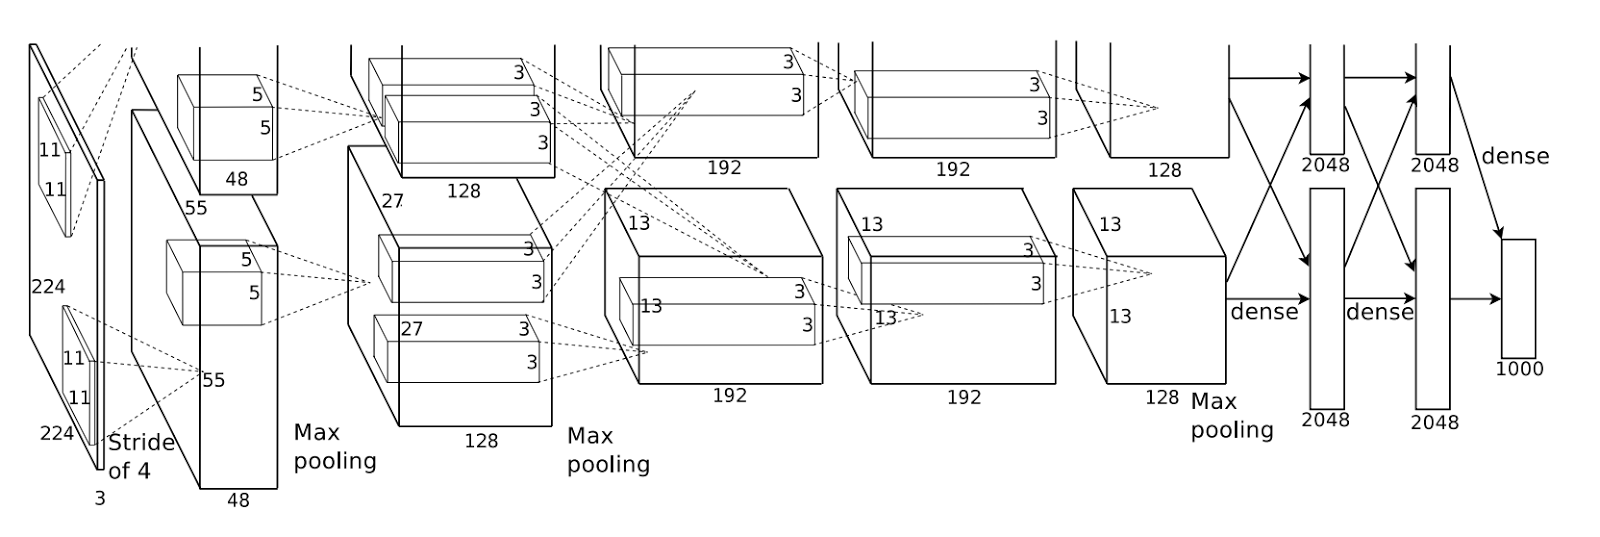
\includegraphics[width=\textwidth]{alexnet.png}
\caption{Architechture of AlexNet.}
\label{fig:alexnet}
\end{figure}

\subsection{Classification}
\label{sec:classification}
The format of the features extracted from an image using the CNN is a vector of length 4096 or 1000. Since each object is now a vector, we can use a traditional classification approach, for example support vector machines (SVM). $C$-Support vector classification (C-SVC)~\citep{boser1992training, cortes1995support} is a form of SVM that includes a penalty on the error term. In this model, the C parameter is added to prevent misclassification in the training set. A large value for $C$ will result in a smaller-margin hyperplane and eventually better classification. On the other hand, a small value of $C$ could lead to misclassified sets, even if the training data is linearly separable. This algorithm also allows the use of kernel functions.

Given our previous experience with python, and the previous use of python in processing and extracting features from the images, we wanted to continue to use python for classification. We chose to use scikit-learn~\citep{scikit-learn}, a mature, open source library that implements multiple machine learning algorithms including classification, regression, and clustering. It has a \emph{sklearn.svm.SVC} library for $C$-support vector classification, an offers multiple kernel methods, as well as a grid search package for optimizing parameters.

There are several ways to configure the C-SVC models. The classification can be changed by specifying the layer of the CNN we use as input (FC6, FC7, FC8), what kernel method we choose for the SVM (linear, RBF, sigmoid, polynomial), and the value of the parameters ($\gamma$, $C$, and degree for polynomial kernels). To test these options we used the grid search functionality of the scikit-learn package to exhaustively determine the best parameters for each kernel/layer combination. For each layer, for each kernel method, we use 10-fold cross validation on the training set to learn the best parameters for the SVM. Then with the best parameters we compared the results for each layer/kernel combination on the training data. From those results we can pick which layer, kernel, and parameter combination we think will have the best result on the test set.

A training and testing split of 2/3 and 1/3 was established at the beginning of experimentation. Each original image was rotated four ways, but all four images were either put in the training or testing set, they were never split into the two groups. The same training and testing split was used for all experiments.
 
 \section{Results}
 \label{sec:results}
As mentioned in Section~\ref{sec:classification}, we applied existing SVM algorithms from SciKit Learn's library to classify the data in our set. For the experiment, we compared the performance of different kernels and feature extraction points from AlexNet. As highlighted in red in Table~\ref{tab:core}, using features extracted from RC6 and RC7 along with the radial basis function kernel both 
provided 100\% accuracy in training. Testing results were consistent with our training results and the \{FC6, RBF\} pair outperformed all other classifiers at 87.8\% accuracy. Therefore, the remainder of this report focuses on \{FC6, RBF\} as the chosen classifier. 

\begin{table}[h]
\caption{Overall accuracy of correctly classified objects from training and testing of SVM models with various kernels. Features were obtained from FC6, FC7 and FC8 exits of AlexNet. (Lin = linear, RBF = radial basis function, Sig = sigmoid, Poly = polynomial)}
\label{tab:core}
\centering
\begin{tabular}{|c|c|c|c|c|c|c|c|c|}\hline
 &  \multicolumn{4}{c|}{Training} & \multicolumn{4}{c|}{Testing}\\\hline
&Lin& RBF&Sig&Poly&Lin& RBF&Sig&Poly\\\hline
FC6&0.942&\cellcolor{SFUred!25}1.000&0.266&0.911&0.821&\cellcolor{SFUred!25}0.878&0.218&0.814\\\hline
FC7&0.876&\cellcolor{SFUred!25}1.000&0.266&0.872&0.788&0.862&0.218&0.804\\\hline
FC8&0.768&0.998&0.266&0.807&0.676&0.843&0.278&0.696\\\hline
\end{tabular}
\end{table}

To better understand the performance of the \{FC6, RBF\} classifier, we present the results on specific labels in Tables~\ref{tab:ripenessMatrix} and~\ref{tab:objectMatrix}. As seen in Table~\ref{tab:ripenessMatrix}, there was no confusion between unripe and overripe bananas. All errors in classifying banana centered around ripe bananas. As for the performance of classifying bananas versus other objects, Table~\ref{tab:objectMatrix} shows that there are more objects that are misidentified than bananas misidentified as other objects. 


	
\begin{table}[h]
\centering
\caption{Confusion matrix on banana ripeness with the \{FC6, RBF\} classifier. }
\label{tab:ripenessMatrix}
\begin{tabular}{|c|c|c|c|c|}\hline
&&\multicolumn{3}{c|}{Predicted}\\\hline
&&Unripe&Ripe&Overripe\\\hline
\multirow{3}{*}{Actual}&Unripe&\cellcolor{SFUred!65}0.913&\cellcolor{SFUred!15}0.095&0.000\\\cline{2-5}
&Ripe&\cellcolor{SFUred!15}0.068&\cellcolor{SFUred!65}0.836&\cellcolor{SFUred!15}0.096\\\cline{2-5}
&Overripe&0.000&\cellcolor{SFUred!15}0.033&\cellcolor{SFUred!65}0.967\\\hline
\end{tabular}
\end{table}

\begin{table}[h]
\centering
\caption{Confusion matrix on banana versus other objects with the \{FC6, RBF\} classifier. }
\label{tab:objectMatrix}
\begin{tabular}{|c|c|c|c|}\hline
&&\multicolumn{2}{c|}{Predicted}\\\hline
&&Banana&Other\\\hline
\multirow{2}{*}{Actual}&Banana&\cellcolor{SFUred!65}0.953&\cellcolor{SFUred!15}0.046\\\cline{2-4}
&Other&\cellcolor{SFUred!15}0.066&\cellcolor{SFUred!65}0.934\\\hline
\end{tabular}
\end{table}

To better understand the incorrectly classified objects from \{FC6, RBF\}, images of correctly and incorrectly classified objects are shown in Figure~\ref{fig:correctVsIncorrect}. Given the size of the data set, it is impractical to present the entire list of correctly or incorrectly identified objects for each class label in the figure. While we have only shown a selected few of the incorrectly classified objects, they are generally representative of the objects that were misclassified.

From the first two rows of Figure~\ref{fig:correctVsIncorrect}, we see that unripe and ripe bananas are often misclassified as each other. This observation correspond with the results shown in Table~\ref{tab:ripenessMatrix}. Furthermore, from the fourth row of Figure~\ref{fig:correctVsIncorrect}, we see that the objects that are misclassified as non-bananas are mostly overripe bananas. This information cannot be directly obtained from Table~\ref{tab:objectMatrix}.

\begin{figure}[h]
\centering
 %%%%%% unripe %%%%%%%%%
  \begin{subfigure}{.123\textwidth}
  \centering
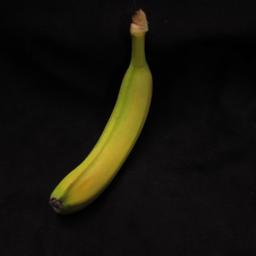
\includegraphics[width=\textwidth]{../results/q_samples/cor_pre.jpg}
\captionsetup{labelformat=empty}
\caption{Unripe}
\end{subfigure}%
\qquad
 \begin{subfigure}{.123\textwidth}
  \centering
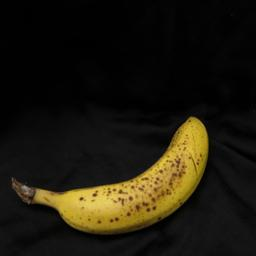
\includegraphics[width=\textwidth]{../results/q_samples/mis_pre/RIPE_1_PRE_1.jpg}
\captionsetup{labelformat=empty}
\caption{}
\end{subfigure}%
  \begin{subfigure}{.123\textwidth}
  \centering
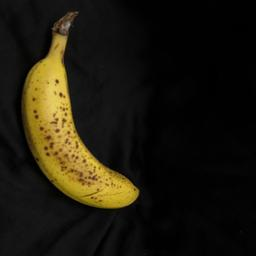
\includegraphics[width=\textwidth]{../results/q_samples/mis_pre/RIPE_1_PRE_3.jpg}
\captionsetup{labelformat=empty}
\caption{}
\end{subfigure}%
  \begin{subfigure}{.123\textwidth}
  \centering
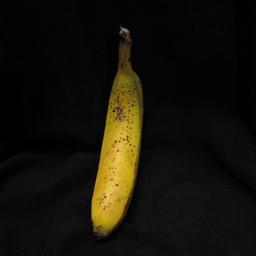
\includegraphics[width=\textwidth]{../results/q_samples/mis_pre/RIPE_1_PRE_4.jpg}
\captionsetup{labelformat=empty}
\caption{}
\end{subfigure}%
  \begin{subfigure}{.123\textwidth}
  \centering
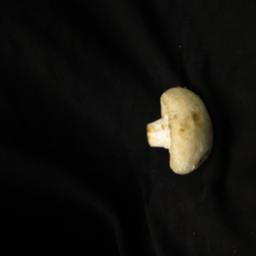
\includegraphics[width=\textwidth]{../results/q_samples/mis_pre/OTHER_1_PRERIPE_1.jpg}
\captionsetup{labelformat=empty}
\caption{}
\end{subfigure}
\vskip .1in
%%%%%% ripe %%%%%%%%%
 \begin{subfigure}{.123\textwidth}
  \centering
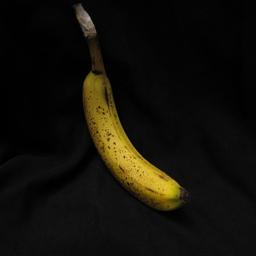
\includegraphics[width=\textwidth]{../results/q_samples/cor_ripe.jpg}
\captionsetup{labelformat=empty}
\caption{Ripe}
\end{subfigure}%
\qquad
 \begin{subfigure}{.123\textwidth}
  \centering
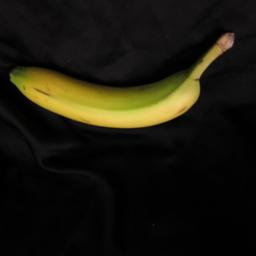
\includegraphics[width=\textwidth]{../results/q_samples/mis_ripe/PRE_2_RIPE_1.jpg}
\captionsetup{labelformat=empty}
\caption{}
\end{subfigure}%
  \begin{subfigure}{.123\textwidth}
  \centering
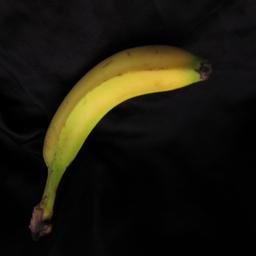
\includegraphics[width=\textwidth]{../results/q_samples/mis_ripe/PRE_2_RIPE_4.jpg}
\captionsetup{labelformat=empty}
\caption{}
\end{subfigure}%
  \begin{subfigure}{.123\textwidth}
  \centering
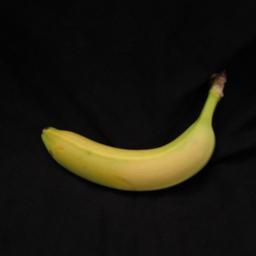
\includegraphics[width=\textwidth]{../results/q_samples/mis_ripe/PRE_2_RIPE_5.jpg}
\captionsetup{labelformat=empty}
\caption{}
\end{subfigure}%
  \begin{subfigure}{.123\textwidth}
  \centering
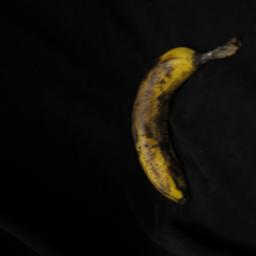
\includegraphics[width=\textwidth]{../results/q_samples/mis_ripe/ROTTEN_2_RIPE_2.jpg}
\captionsetup{labelformat=empty}
\caption{}
\end{subfigure}
\vskip .1in
 %%%%%% overripe %%%%%%%%%
  \begin{subfigure}{.123\textwidth}
  \centering
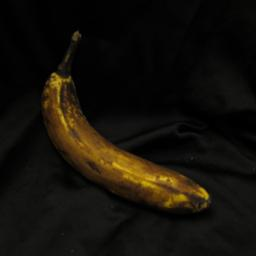
\includegraphics[width=\textwidth]{../results/q_samples/cor_rotten.jpg}
\captionsetup{labelformat=empty}
\caption{Overripe}
\end{subfigure}%
\qquad
 \begin{subfigure}{.123\textwidth}
  \centering
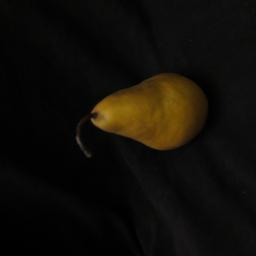
\includegraphics[width=\textwidth]{../results/q_samples/mis_rotten/OTHER_0_ROTTEN_1.jpg}
\captionsetup{labelformat=empty}
\caption{}
\end{subfigure}%
  \begin{subfigure}{.123\textwidth}
  \centering
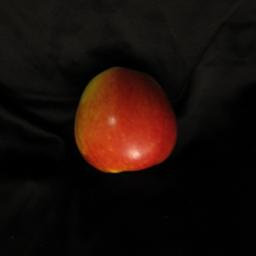
\includegraphics[width=\textwidth]{../results/q_samples/mis_rotten/OTHER_0_ROTTEN_2.jpg}
\captionsetup{labelformat=empty}
\caption{}
\end{subfigure}%
  \begin{subfigure}{.123\textwidth}
  \centering
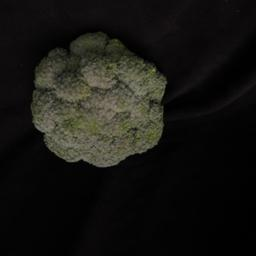
\includegraphics[width=\textwidth]{../results/q_samples/mis_rotten/OTHER_0_ROTTEN_3.jpg}
\captionsetup{labelformat=empty}
\caption{}
\end{subfigure}%
  \begin{subfigure}{.123\textwidth}
  \centering
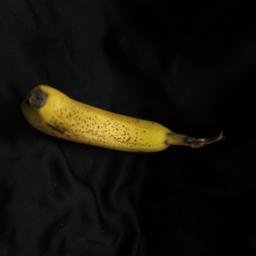
\includegraphics[width=\textwidth]{../results/q_samples/mis_rotten/RIPE_0_ROTTEN_2.jpg}
\captionsetup{labelformat=empty}
\caption{}
\end{subfigure}
 \vskip .1in
 %%%%%% non banana %%%%%%%%%
 \begin{subfigure}{.123\textwidth}
  \centering
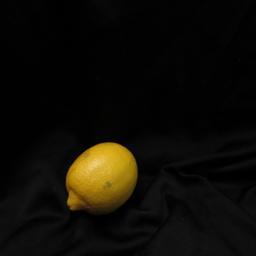
\includegraphics[width=\textwidth]{../results/q_samples/cor_other.jpg}
\captionsetup{labelformat=empty}
\caption{Other}
\end{subfigure}%
\qquad
 \begin{subfigure}{.123\textwidth}
  \centering
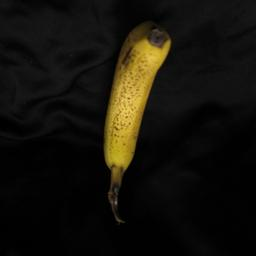
\includegraphics[width=\textwidth]{../results/q_samples/mis_other/RIPE_3_OTHER_2.jpg}
\captionsetup{labelformat=empty}
\caption{}
\end{subfigure}%
  \begin{subfigure}{.123\textwidth}
  \centering
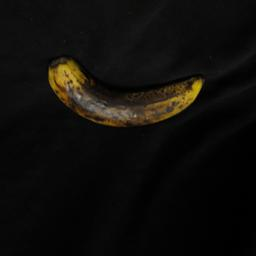
\includegraphics[width=\textwidth]{../results/q_samples/mis_other/ROTTEN_3_OTHER6.jpg}
\captionsetup{labelformat=empty}
\caption{}
\end{subfigure}%
  \begin{subfigure}{.123\textwidth}
  \centering
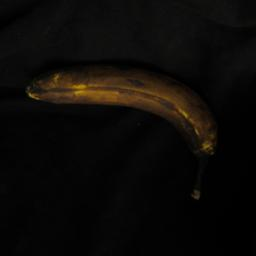
\includegraphics[width=\textwidth]{../results/q_samples/mis_other/ROTTEN_3_OTHER_3.jpg}
\captionsetup{labelformat=empty}
\caption{}
\end{subfigure}%
  \begin{subfigure}{.123\textwidth}
  \centering
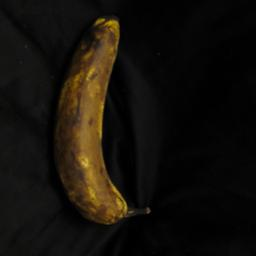
\includegraphics[width=\textwidth]{../results/q_samples/mis_other/ROTTEN_3_OTHER_6.jpg}
\captionsetup{labelformat=empty}
\caption{}
\end{subfigure}
\caption{Samples of correctly classified data from each class are presented in the first column. For each row, the remaining columns contain samples of incorrectly classified objects that have been given the same label as the object in the first column. }
\label{fig:correctVsIncorrect}
\end{figure}
\section{Discussion}
\label{sec:conclusion}

Our method outperformed  the performance of~\citet{saad2009recognizing} in classifying banana ripeness with significantly larger data set. In addition to improving the accuracy of classification over previous works, we also added detection of non-banana objects as an extra feature in this project. 

There are several future directions for this project. Since we used a pre-trained model to extract features from our data set, we can improve the feature extraction process by training the model and fine tuning the parameters of the model. Features extracted from a refined model should provide more representative feature sets that would improve the classification results.

Aside from simply detecting ripeness of bananas, the core idea of this algorithm could be expanded for ripeness detection for other fruits and vegetables. This project can also be expanded into other environment. We aim to implement this as an application for mobile operating systems. A mobile app that could detect fruit ripeness through computer vision is an useful tool for individuals who have impaired senses. From an industrial point of view, this program could be essential in automatic large scale sorting.

The data set used in this project as well as the accompanying code are available at bit.ly/BananaRipe.

\subsubsection*{Acknowledgments}
We thank our TA Zhiwei (Lucas) Deng and for his guidance on using Caffe as well as AlexNet. We also thank Dr. Mori for his insights on solving this problem. 

\subsubsection*{Contributions}
Contributions were as follows. Kyle Demeule: Creation and processing of data set, feature extraction with Caffe, SVM implementation and optimization, editing of report. Bernard Chan: SVM implementation, literature review, poster creation, and majority of report. Saeed Soltani: SVM optimization, PCA research, literature review, and report contributions.
 
\renewcommand\refname{\vskip -.75cm}
\subsubsection*{References}

   \bibliography{report}		    
   \bibliographystyle{plainnat}
\end{document}
